% Toolbar icon: merge coincident nodes — two nodes with arrows converging onto a
% single (merged) node in the middle.
\documentclass[tikz,border=2mm]{standalone}
\usetikzlibrary{arrows.meta,calc,shapes.geometric}
\begin{document}
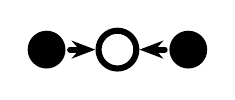
\begin{tikzpicture}[line width=2.2pt, line cap=round, line join=round, >=Stealth, x=1mm,y=1mm]
  \fill (-9,0) circle (2.4);
  \fill (9,0) circle (2.4);
  \draw[line width=2.2pt,-{Stealth[length=3mm]}] (-6,0) -- (-2.8,0);
  \draw[line width=2.2pt,-{Stealth[length=3mm]}] (6,0) -- (2.8,0);
  \draw[line width=2.2pt] (0,0) circle (2.4);
\end{tikzpicture}
\end{document}
